\documentclass[master=cws,masteroption=gs]{kulemt}
\setup{title={Configuratieafhankelijkheden gebruiken om gedistribueerde applicaties effici\"ent te beheren in een hybride cloud},
  author={Harm De Weirdt},
  promotor={Prof.\,dr.\,ir.\ Wouter Joosen},
  assessor={Ir.\,W. Eetveel\and W. Eetrest}, %TODO
  assistant={Ir.\ Bart Vanbrabant}}
% De volgende \setup mag verwijderd worden als geen fiche gewenst is.
\setup{filingcard,
    translatedtitle={Configuratieafhankelijkheden gebruiken om gedistribueerde applicaties effici\"ent te beheren in een hybride cloud},
  udc=T134, %TODO: checken
  shortabstract={
      \begin{description}
          \item[Context] \hfill \\ Om IT infrastructuren efficient te beheren wordt er gebruik gemaakt van configuratiebeheergereedschappen. Deze gereedschappen zijn model gebaseerd, waarbij het model de gewenste toestand van de configuratie beschrijft. Om de configuratie door te voeren wordt de gewenste toestand vergeleken met de huidige toestand en worden de nodige acties afgeleid die nodig zijn om de infrastructuur in die gewenste toestand te brengen. Huidge systemen zijn reeds in staat om eenvoudige afhankelijkheden af te leiden. Bijvoorbeeld dat een service eerst geïnstalleerd moet worden voordat die service gestart kan worden. Wat ontbreekt is afhankelijkheden tussen services op verschillende systemen in rekening brengen.
        \item[Doel] \hfill \\Het doel van deze thesis is onderzoeken hoe afhankelijkheden in een configuratiemodel gebruikt kunnen worden om de initiele configuratie en mogelijke herconfiguraties van een hybrid cloud zo efficient mogelijk uit te voeren.
        \item[Onderzoeksvragen] \hfill \\
            \begin{enumerate}
                \item Hoe kunnen afhankelijkheden in een configuratiemodel gebruikt worden om veranderingen zo snel mogelijk uit te rollen?
                \item Kan de gevraagde tijd gesimuleerd worden in functie van het configuratie model?
            \end{enumerate}
        \item[Uitwerking] \hfill \\
            \begin{description}
                \item[Fase 1] Vertrouwd geraken met het configuratiebeheergereedschap
                \item[Fase 2] Onderzoeken van bestaande configuratiemodellen
                \item[Fase 3] Implementeren van een oplossing
                \item[Fase 4] Valideren van de oplossing door middel van de configuratiemodellen op een private en publieke cloud en een simulator
            \end{description}
    \end{description}
}}
% Verwijder de "%" op de volgende lijn als je de kaft wil afdrukken
%\setup{coverpageonly}
% Verwijder de "%" op de volgende lijn als je enkel de eerste pagina's wil
% afdrukken en de rest bv. via Word aanmaken.
%\setup{frontpagesonly}

% Kies de fonts voor de gewone tekst, bv. Latin Modern
\setup{font=lm}

% Hier kun je dan nog andere pakketten laden of eigen definities voorzien

% Tenslotte wordt hyperref gebruikt voor pdf bestanden.
% Dit mag verwijderd worden voor de af te drukken versie.
\usepackage[pdfusetitle,colorlinks,plainpages=false]{hyperref}

\usepackage{todonotes}

\begin{document}

\begin{preface}
  Dit is mijn dankwoord om iedereen te danken die mij bezig gehouden heeft.
  Hierbij dank ik mijn promotor, mijn begeleider en de voltallige jury.
  Ook mijn familie heeft mij erg gesteund natuurlijk.
\end{preface}

\tableofcontents*

\begin{abstract}
  In dit \texttt{abstract} environment wordt een al dan niet uitgebreide
  samenvatting van het werk gegeven. De bedoeling is wel dat dit tot
  1~bladzijde beperkt blijft.

\end{abstract}

% Een lijst van figuren en tabellen is optioneel
%\listoffigures
%\listoftables
% Bij een beperkt aantal figuren en tabellen gebruik je liever het volgende:
\listoffiguresandtables

\mainmatter

\chapter{Inleiding}
\label{inleiding}
%%%%%%%%%%%%%%%%%%%%%%%%%%%%%%%%%%%%%%%%%%%%%%%%%%%%%
%          Waarom configuratiemanagement?           %
%%%%%%%%%%%%%%%%%%%%%%%%%%%%%%%%%%%%%%%%%%%%%%%%%%%%%
Configuratiebeheergereedschappen zijn ontwikkeld om het leven van systeembeheerders makkelijker te maken.
De serverinfrastructuren die ze moeten onderhouden worden steeds uitgebreider en complexer.
Manueel elke server configureren kost niet alleen teveel tijd maar is ook erg foutgevoelig.
Het gebruik van scripts is al een stap in de goede richting maar is nog steeds niet voldoende.
Als bijvoorbeeld ssh gebruikt wordt om een reeks servers up te daten en \'e\'en ervan is niet beschikbaar is er plots een verschil tussen systemen die eigenlijk dezelfde configuratie zouden moeten hebben. \todo{Herschrijven}

Een andere manier om een verzameling gelijkaardige machines van hun initi\"ele configuratie te voorzien is het gebruik van images.
Daarbij wordt eerst \'e\'en machine manueel geconfigureerd en daarna de volledige set-up gekloond naar de rest van de servers.
Deze methode werkt niet meer voor het verdere onderhoud van de configuraties.
%http://sysadvent.blogspot.be/2011/12/day-19-why-use-configuration-management.html

%%%%%%%%%%%%%%%%%%%%%%%%%%%%%%%%%%%%%%%%%%%%%%%%%%%%%
%          Overgaan naar de cloud                   %
%%%%%%%%%%%%%%%%%%%%%%%%%%%%%%%%%%%%%%%%%%%%%%%%%%%%%
Dit onderhoudsprobleem komt nog prominenter voor als de infrastructuur niet lokaal maar in de cloud gehost wordt.
Een groot voordeel van werken in de cloud is de flexibiliteit waarmee servers kunnen toegevoegd en weggenomen kunnen worden.
Dit proces gebeurt vaak zelfs automatisch waardoor manuele configuratie helemaal geen optie meer is. \todo{source?}
In een dergelijke omgeving is een tool die uit zichzelf de volledige infrastructuur kan beheren bijna een noodzaak.
Configuratiebeheergereedschappen (of CMS: Configuration Management Software, vanaf nu zal deze term gebruikt worden) zoals
IMP\footnote{http://people.cs.kuleuven.be/~bart.vanbrabant/impdoc/index.html},Puppet\footnote{http://puppetlabs.com/}, CFEngine\footnote{http://cfengine.com/},\ldots laten toe op een effici\"ente manier IT infrastructuren op te zetten en onderhouden.

%%%%%%%%%%%%%%%%%%%%%%%%%%%%%%%%%%%%%%%%%%%%%%%%%%%%%
%          Werking huidige tools                    %
%%%%%%%%%%%%%%%%%%%%%%%%%%%%%%%%%%%%%%%%%%%%%%%%%%%%%
De gebruiker van een dergelijke tool specifi\"eert eerst een model dat de gewenste toestand van de volledige infrastructuur beschrijft.
Dit model bestaat uit een oplijsting van machines met de gewenste aanwezige resources (bestanden, mappen, services,\ldots) die ze moeten aanbieden.
%Dit model is zo bij de huidige tools, niet echt bij IMP
Een eenvoudige voorbeeldconfiguratie is de LAMP-stack: een Linuxinstallatie met daarop een Apache webserver, de MySQL databaseservice en PHP.

Bij het uitrollen van een configuratie (een "deployment run") inspecteert de CMS de huidige toestand van elke machine en vergelijkt ze met de gewenste toestand.
Als er een verschil is maakt de CMS de nodige aanpassingen, indien niet onderneemt ze geen actie.
De beheerder van de verzameling systemen moet dus na het opstellen van de initi\"ele configuratie zelf geen stappen meer ondernemen om te verzekeren dat de gewenste situatie bereikt wordt.
Als er later nog aanpassingen moeten gebeuren moet enkel het model aangepast worden en een nieuwe deployment run gestart worden, manueel inloggen op elke server is niet meer nodig.


%%%%%%%%%%%%%%%%%%%%%%%%%%%%%%%%%%%%%%%%%%%%%%%%%%%%%
%          Dependencies gebruiken gaat beter        %
%%%%%%%%%%%%%%%%%%%%%%%%%%%%%%%%%%%%%%%%%%%%%%%%%%%%%
Een belangrijk aspect van elk gedistribueerd systeem zijn de afhankelijkheden die bestaan tussen de verschillende delen van dat systeem.
In het voorbeeld van de LAMP-stack heeft de webserver naast PHP-mogelijkheden ook een werkende database nodig, anders kan deze niet alle functionaliteit aanbieden.
\begin{figure}
    \label{fig:lamp_dep}
    \begin{center}
    \includegraphics[width=0.6\textwidth]{images/lamp_dep.png}
    \caption{Grafische voorstelling van de afhankelijkheden binnen een LAMP-stack}
    \end{center}
\end{figure}
Als deze afhankelijkheden niet gespecifi\"eerd worden in het model kan de CMS er ook geen rekening mee houden.
De tool kan dus het model in een foute volgorde verwerken: eerst de webserver, dan php en uiteindelijk de database.
De webserver zal bij het opstarten proberen te verbinden met de database, maar deze is nog niet online.
Een op het eerste zicht succesvolle deployment run kan dus leiden tot een configuratie die niet volledig werkt.

In vergelijking met de beginsituatie is de toestand van de setup na \'e\'en run wel al minder afwijkend van de gewenste situatie:
de CMS zal nooit aanpassingen maken die zorgen voor een configuratie die verder afwijkt van het model dan voorheen.
Na een paar iteraties zal uiteindelijk altijd de gewenste configuratie bereikt worden.
Het aantal iteraties is afhankelijk van de hoeveelheid afhankelijkheden die bestaan maar niet aanwezig zijn in het model.
De kans bestaat wel altijd dat met wat geluk de CMS een willekeurige maar effici\"ente volgorde kiest.
\begin{figure}
    \label{fig:convergentie}
    \begin{center}
    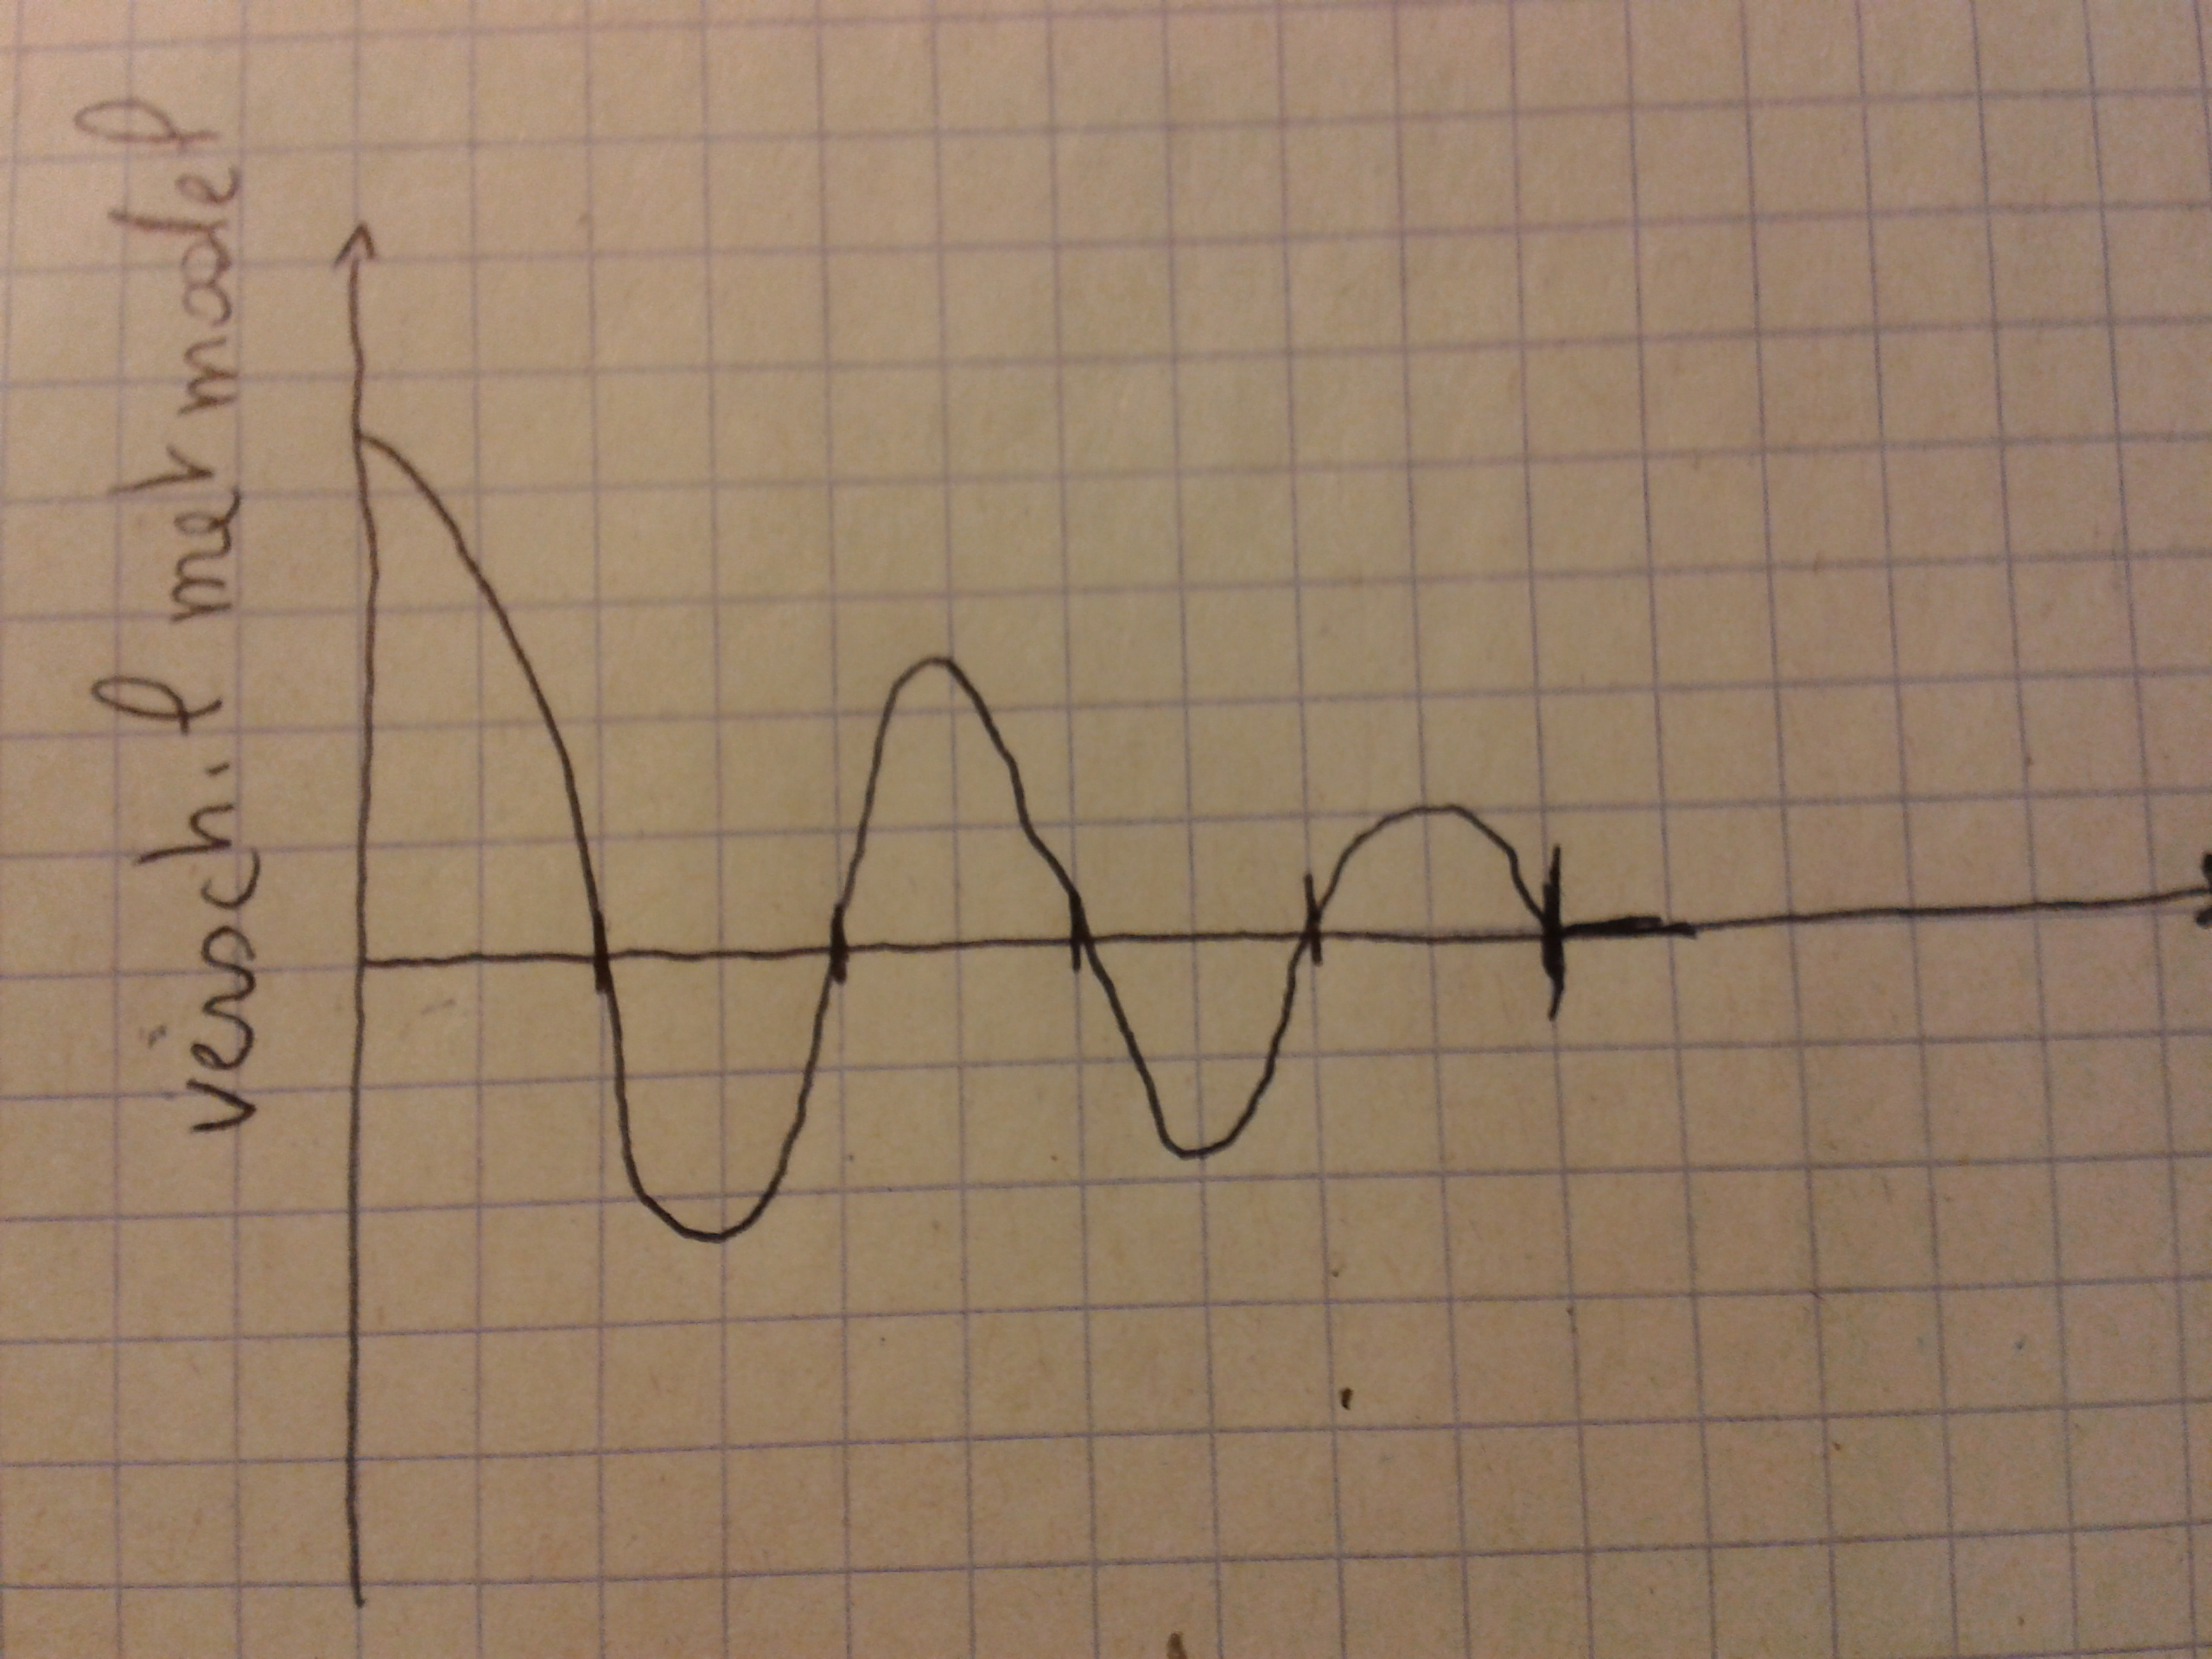
\includegraphics[width=0.6\textwidth]{images/convergentie.png}
    \caption{Grafische voorstelling van de convergentie na een reeks deployment runs.}
    \end{center}
\end{figure}

%CMS laat vaak toe om logisch samenhorende basisobjecten te verzamelen en   
Databases en webserver zijn abstracties die bestaan uit een verzameling basisobjecten zoals bestanden, packages en services.
Tussen deze objecten bestaan er natuurlijk ook afhankelijkheden, bijvoorbeel tussen een bestand en de map waarin het staat:
als de CMS eerst probeert het bestand te cree\"eren en dan pas de map zal de deployment run slechts gedeeltelijk slagen want een bestand kan niet bestaan zonder zijn parent folder.
\begin{figure}
    \label{fig:file_dir_dep}
    \begin{center}
    \includegraphics[width=0.6\textwidth]{images/file_dir_dep.png}
    \caption{Grafische voorstelling van de afhankelijkheid tussen een bestand en zijn parent folder}
    \end{center}
\end{figure}
\todo{Hier al eventual consistency vermelden/verwijzen?}

We kunnen dus concluderen dat het vermelden van dependencies in het model het uitrolprocess significant kan verbeteren: als alle afhankelijkheden vermeld zijn is er maar 1 deployment run nodig.
\todo{snelheid nog niet vermeld. Meerdere deployments onnodig maken.}
\todo{Belang: correct gebeuren is van groot belang}

%%%%%%%%%%%%%%%%%%%%%%%%%%%%%%%%%%%%%%%%%%%%%%%%%%%%%
%          Dependencies met huidige tools           %
%%%%%%%%%%%%%%%%%%%%%%%%%%%%%%%%%%%%%%%%%%%%%%%%%%%%%
De huidige CMS laten toe om op het niveau van bestanden, packages en services afhankelijkheden te specifi\"eren.
Bij het uitrollen van een model wordt dan een volgorde opgelegd waarmee de verschillende objecten verwerkt worden.

De tools die momenteel beschikbaar zijn compileren tijdens de deployment voor elke machine hun deel van het model.
Elke machine krijgt dus informatie over wat hijzelf doet maar kan geen rekening houden met wat er op andere machines gebeurt.
Afhankelijkheden binnen \'e\'en machine verwerken is dus geen probleem maar afhankelijkheden tussen verschillende machines zijn niet mogelijk. \todo{Vermelden van workarounds}
De tools die momenteel beschikbaar zijn kunnen dus het hierboven vermelde probleem van een webserver en een database niet oplossen.
%%%%%%%%%%%%%%%%%%%%%%%%%%%%%%%%%%%%%%%%%%%%%%%%%%%%%
%          Dependencies met IMP                     %
%%%%%%%%%%%%%%%%%%%%%%%%%%%%%%%%%%%%%%%%%%%%%%%%%%%%%
IMP (Infrastructure Management Platform) is een nieuwe tool die momenteel nog in ontwikkeling is.
Een andere aanpak tijdens het deployen van een model laat toe afhankelijkheden tussen hoog-niveau objecten te specifi\"eren:
in tegenstelling tot de vorige tools krijgt elke machine het volledige model ter beschikking en niet alleen zijn eigen deel.
Dit laat de machines toe om rekening te houden met afhankelijkheden tussen eigen objecten en die op een andere machine.

%%%%%%%%%%%%%%%%%%%%%%%%%%%%%%%%%%%%%%%%%%%%%%%%%%%%%
%          Probleem/doelstelling                    %
%%%%%%%%%%%%%%%%%%%%%%%%%%%%%%%%%%%%%%%%%%%%%%%%%%%%%
De doelstelling van deze thesis is een effici\"ente manier vinden om een configuratiemodel uit te rollen.
Effici\"ent slaat hier vooral op het vermijden van extra deployment runs door rekening te houden met al dan niet impliciete afhankelijkheden.

%%%%%%%%%%%%%%%%%%%%%%%%%%%%%%%%%%%%%%%%%%%%%%%%%%%%%
%          Kort: hoe oplossing + resultaten         %
%%%%%%%%%%%%%%%%%%%%%%%%%%%%%%%%%%%%%%%%%%%%%%%%%%%%%

\chapter{Analyse van het probleem}
\label{chapter:1}
In dit deel wordt er dieper ingegaan op de probleemstelling.
Voor elke soort afhankelijkheid komt er een korte uitleg en daarna \'e\'en of meerdere heuristieken die toepasbaar zijn.

\section{Soorten afhankelijkheden}
\label{section:soorten_afhankelijkheden}
Zoals in de inleiding duidelijk werd bestaan er verschillende categori\"en van afhankelijkheden.
Elke categorie verschilt in moeilijkheid en aanpak. 

\subsection{Afhankelijkheden tussen bestanden en mappen}
\label{subs:bestanden_en_mappen}
#Hier gaat het over de afhankelijkheid tussen een bestand en de map waarin het staat.
#Een bestand kan niet bestaan zonder een map dus een heuristiek die elk bestand afhankelijk maakt van zijn parent folder is toepasselijk.
Tussen bestanden en mappen bestaat er zonder twijfel een sterke afhankelijkheid: een bestand kan helemaal niet bestaan zonder een map.
De eerste heuristiek die werd gebruikt in IMP is er een die voor elk bestand de "parent folder" opzoekt in het model en een afhankelijkheid toevoegd als deze gevonden wordt.
Als de map niet vermeld wordt in het model wordt deze ook niet toegevoegd omdat dit ongewenste gevolgen kan hebben. \todo{Welke?}
\missingfigure{Visuele voorstelling}

\subsection{Afhankelijkheden bij service stacks}
\label{subs:service_stacks}
Net zoals tussen bestanden en mappen is er een sterke afhankelijkheid tussen packages, services en hun eventuele configuratiebestanden:
een service kan niet gestart worden als zijn package niet ge\"installeerd is en zal niet correct werken zonder een juiste configuratie.
Een gelijkaardige heuristiek als die van bestanden en mappen kan er dus voor zorgen dat automatisch tussen de correcte afhankelijkheden worden ge\"introduceerd.
\\
"Service stack" is een eigen term die ik gegeven heb aan een verzameling van een package en een service (en mogelijks ook een configuratiebestand).
De verzameling wordt bepaald door te zoeken naar resources die binnen dezelfde scope gedefini\"eerd zijn.

\subsection{Afhankelijkheden door relaties}
\label{subs:relaties}
IMP laat toe in het model relaties tussen hoog-niveau objecten te specifi\"eren.
Sommige relaties, zoals "x [1:] -- [0:] y" impliceren dat y niet kan bestaan zonder een instantie van x.
Zo bekomen we een heuristiek die de afhankelijkheid tussen x en y toevoegt aan het model.

\subsection{Afhankelijkheden tussen machines}
In dit hoofdstuk wordt verder ingegaan op hoe afhankelijkheden tussen verschillende machines verwerkt worden.
Het belangrijkste punt is hoe hoog-niveau relaties en afhankelijkheden vertaalt worden naar dependencies op de lagere niveaus.

\section{Besluit van dit hoofdstuk}
 %Analyse van het probleem
\chapter{Evaluatie}
\label{hoofdstuk:2}

\section{Besluit van dit hoofdstuk}
 %Evaluatie
\chapter{Besluit}
\label{sec:besluit}

\section{Gerelateerd werk}
\todo{verwijzen naar overzichtspaper}
Cloud Resource Orchestration: A Data-Centric Approach: andere aanpak om te vermijden dat inconsistente configuraties bereikt worden.
Datacentrische aanpak (declaratief) itt tot andere tools die heel imperatief werken (bvb ansible)

\todo{IBM}

\section{Verder werk}
%Meer use cases%
Een eerste onderzoeksrichting betreft de heuristieken.
Niet alleen worden deze beter nog in andere use cases gebruikt om hun validiteit verder te bevestigen, nieuwe use cases kunnen ook leiden tot nieuwe heuristieken.

De heuristieken kunnen mogelijks ook gebruikt worden als onderdeel van een intelligente autocompletetool. 
Een dergelijke tool stelt de gebruiker voor om vereisten tussen resources binnen een stack toe te voegen, of suggereert om bepaalde relaties als afhankelijk te specificeren.

%kijken welke subset van deps nu echt nodig is.%
Verder onderzoek kan ook pogen de minimale set vereisten te defini\"eren die nodig is om een model correct uit te rollen.
De heuristieken die voortkomen uit dit onderzoek voegen liever een extra vereiste toe dan geen.
Deze aanpak is goed zolang er geen incorrecte of overbodige vereisten worden toegevoegd, maar elke vereiste moet verwerkt worden door IMP.
Dit zorgt voor een kleine verhoging in de uitvoertijd.
Een minimale set vereisten kan dus een positief effect hebben op de totale uitroltijd.

%Deletes%
Een derde richting die verder onderzocht kan worden is hoe IMP (of CMS in het algemeen) kan omgaan met verschillende tussen opeenvolgende versies van een configuratiemodel.
Momenteel stopt alle CMS dan met het onderhoud van die resource. 
In sommige gevallen kan dit ongewenste gevolgen hebben: een database die online blijft maar een niet meer geupdated wordt is een veiligheidsrisico.
De service stoppen als ze niet meer in het model vermeld staat zou hier een betere optie zijn.
Mogelijks leidt dit zelfs tot andere resources die overbodig worden, zoals een database die enkel gebruikt door een webserver.
Als de webserver uitgeschakeld wordt kan het wenselijk zijn om automatisch ook de databaseserver stop te zetten.
Dit soort acties zijn mogelijk in IMP omdat in het model de relaties staan die aanwezig zijn in de opstelling.


% Indien er bijlagen zijn:
\appendixpage*          % indien gewenst
\appendix
\chapter{Code van de heuristieken}
\label{app:code}
\section{Bestanden en mappen}
\begin{minipage}{\textwidth}
\begin{lstlisting}[language=Python]
def dir_before_file(model, resources):
    for _id, resource in resources.items():
        model = resource.model
        res_class = model.__class__
        if model.__module__ == "std" and (res_class.__name__ == "File" or res_class.__name__ == "Directory"):
            host = model.host
 
            for dir in host.directories:
                dir_res = Resource.get_resource(dir)
                if dir_res is not None and os.path.dirname(resource.path) == dir_res.path:
                    if dir_res.id not in resource.requires:
                        resource.requires.add(dir_res.id)
\end{lstlisting}
\end{minipage}

\section{Services, packages en configuratiebestanden}
\subsection{Methode 1}
\begin{minipage}{\textwidth}
\begin{lstlisting}[language=Python]
TODO: herschrijven
\end{lstlisting}
\end{minipage}

\subsection{Methode 2}
\begin{minipage}{\textwidth}
\begin{lstlisting}
def scope_dependencies(model, resources):
    srv_stacks = find_srv_stacks(resources)
    deps_per_stack = [] 
    for stack in srv_stacks:
        deps_per_stack.append(setup_stack_deps(stack))
 
def find_srv_stacks(resources):
    stacks = []
    for res in resources.values():
        scope_pkg = []
        scope_cfg = []
        scope_srv = []
        model_instance = res.model
        instance_scope = model_instance.__scope__
        scope_vars = instance_scope.variables()
        scope_cfg = [x.value for x in scope_vars if x.value.__class__.__name__ == "File"]
        scope_srv = [x.value for x in scope_vars if x.value.__class__.__name__ == "Service"]
        scope_pkg = [x.value for x in scope_vars if x.value.__class__.__name__ == "Package"]
 
        if scope_srv and (scope_pkg or scope_cfg):
            stacks.append({'pkg': scope_pkg, 'srv': scope_srv, 'cfg': scope_cfg})
 
    return stacks
 
def setup_stack_deps(stack):
    deps = 0
    for srv in stack['srv']:
        srv = Resource.get_resource(srv)
        for pkg in stack['pkg']:
            pkg = Resource.get_resource(pkg)
            if pkg.id not in srv.requires:
                srv.requires.add(pkg.id)
                deps = deps + 1
        for cfg in stack['cfg']:
            cfg = Resource.get_resource(cfg)
            if cfg.id not in srv.requires:
                srv.requires.add(cfg.id)
                deps = deps + 1
    for cfg in stack['cfg']:
        cfg = Resource.get_resource(cfg)
        for pkg in stack['pkg']:
            pkg = Resource.get_resource(pkg)
            if pkg.id not in cfg.requires:
                cfg.requires.add(pkg.id)
                deps = deps + 1
    return deps

\end{lstlisting}
\end{minipage}

\section{Resources met gelijkaardige namen}
\begin{minipage}{\textwidth}
\begin{lstlisting}
def name_dependencies(model, resources):
    deps = 0
    for _id, res in resources.items():
        similar_resources = []
        res_model = res.model
        if res_model.__module__ == "std" and res_model.__class__.__name__ == "Service":
            for other_id, other_res in resources.items():
                similar_reg = re.compile("std::File.*%s.*%s.*" % (res.model.host.name, res.name))
                if other_res.model.__class__.__name__ == "File" and similar_reg.match(str(other_id)):
                    similar_resources.append(other_res)
            
            for similar_res in similar_resources:
                if similar_res.id not in res.requires:
                    res.requires.add(similar_res.id)
 
        if res_model.__module__ == "std" and res_model.__class__.__name__ == "Package":
            pkg_name = ''.join(i for i in res.name if not i.isdigit())
            pkg_name = pkg_name.split("-")[0]
            for other_id, other_res in resources.items():
                similar_reg = re.compile("std::File.*%s.*%s.*" % (res.model.host.name, pkg_name))
                if other_res.model.__class__.__name__ == "File" and similar_reg.match(str(other_id)):
                    similar_resources.append(other_res)
            
            for similar_res in similar_resources:
                if res.id not in similar_res.requires and similar_res not in res.requires:
                    similar_res.requires.add(res.id)
\end{lstlisting}
\end{minipage}

\section{Afhankelijkheden door relaties}
\begin{minipage}{\textwidth}
\begin{lstlisting}
def use_rel_multiplicity(model, resources):
    added = 0
    for lib in model.get_scopes():
        for concept in lib.variables():
            if concept.get_name().startswith("Entity"):
                for attr_name in concept.value.get_all_attribute_names(): #anders niet de attr vd parents
                    attr_value = concept.value.get_attribute(attr_name)
                    if hasattr(attr_value, "end"): #Kijk of het een relatie is
                        attr_end = attr_value.end
                        if attr_end.low >= 1 and attr_end.end.low == 0 and not attr_value.depends:
                            added = added + 1
                            attr_value.depends = True 
\end{lstlisting}
\end{minipage}

\section{Vereisten door afhankelijkheden}
\begin{minipage}{\textwidth}
\begin{lstlisting}
def use_relations(model, resources):
    depends = 0
    added = 0
    for lib in model.get_scopes():
        for concept in lib.variables():
            if concept.get_name().startswith("Entity"):
                concept_services = get_services(concept)
                if concept_services is not None: #Als er geen services zijn moeten er sowieso geen deps opgesteld worden
                    for attr_name in concept.value.get_all_attribute_names(): #anders niet de attr vd parents
                        attr_value = concept.value.get_attribute(attr_name)
                        if hasattr(attr_value, "end"): #Kijk of het een relatie is
                            if attr_value.end.depends: #Kijk of het concept afhankelijk is vd andere kant
                                depends = depends + 1
                                for instance in concept.value: #Voor elke instantie v/h concept de deps opstellen
                                    req_concepts = getattr(instance, attr_name)
                                    req_resources = []
                                    if hasattr(req_concepts, 'append'): #Check if QList
                                        for req_concept in req_concepts:
                                            for srv in get_child_services(req_concept):
                                                req_resources.append(srv)
                                    else:
                                        for srv in get_services(req_concepts):
                                                req_resources.append(srv)
                                    for req_res in req_resources:
                                        for service in concept_services:
                                            if req_res not in service.requires and req_res.state != "stopped":
                                                service.requires.add(req_res)

def get_child_services(object):
    services = []
    for child_res in object._childeren:
            if child_res.__module__ == "std" and child_res.__class__.__name__ == "Service":
                services.append(Resource.get_resource(child_res))
    return services
 
def get_services(concept):
    found_services = []
    
    if hasattr(concept, "value"):
        for instance in concept.value:
            if concept.__module__ == "std" and concept.__class__.__name__ == "Service":
                found_services.append(Resource.get_resource(concept))
             
            if hasattr(instance, "_childeren"):
                found_services.extend(get_child_services(instance))
                
    if hasattr(concept, "_childeren"):
                found_services.extend(get_child_services(concept))                
 
    return set(found_services)
\end{lstlisting}
\end{minipage}


\backmatter
% Na de bijlagen plaatst men nog de bibliografie.
% Je kan de  standaard "abbrv" bibliografiestijl vervangen door een andere.
\bibliographystyle{abbrv}
\bibliography{referenties}

\end{document}

%%% Local Variables: 
%%% mode: latex
%%% TeX-master: t
%%% End: 
